%%%% File: rulers-small.tex
%%%% Provides 24  70-cm rulers at centimeter and millimeter scale, all numbered 
%%%% Author: Ricardo Hernández, with much help from Qrrbrbirlbel
%%%% (http://tex.stackexchange.com/users/16595/qrrbrbirlbel) and the kind people
%%%% at TeX.Stackexchange. See: http://tex.stackexchange.com/a/121490/3731
%%%% Date: Saturday June 29, 2013
%%%% The rulers will be used on top and on one side of a flume at the University
%%%% of South Carolina, and on a bunch of mounts placed atop the flume. It will
%%%% be printed in low tack transparent adhesive paper. 


\documentclass[tikz,convert=false,12pt]{standalone}


%%%% Redefine the default font face to be sans serif, specifically a helvetica
%%%% clone called TeX Gyre Heros. 
\usepackage{tgheros}
\renewcommand*\familydefault{\sfdefault} 
\usepackage[T1]{fontenc}

% \usetikzlibrary{external} 
% \tikzexternalize

\begin{document}

%%%% Change the order of the TikZ coordinate system so that the rulers go from
%%%% right to left, at centimeter scale. Any unit not specified is multiplied by
%%%% 1 cm. This allows some fancy scaling. 
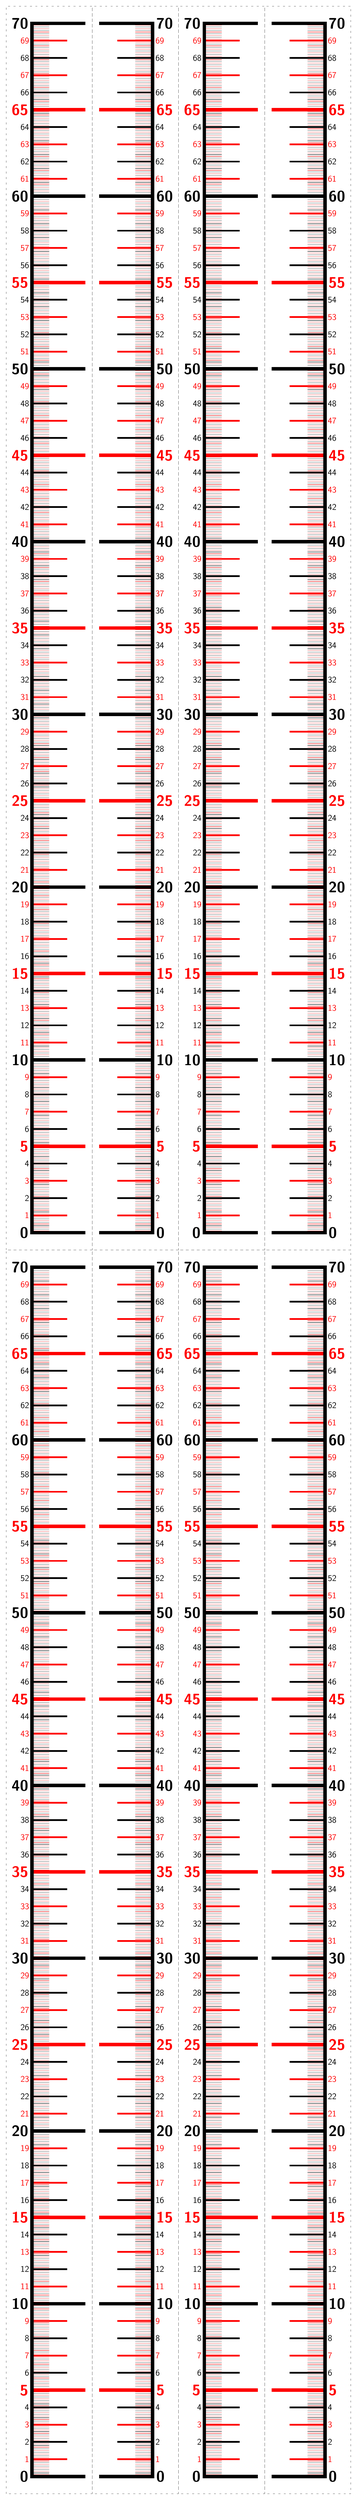
\begin{tikzpicture}[x=1mm,line cap=rect]

  
  %%%% We need 12 rulers, mirrored, for a grand total of 24 rulers. This script
  %%%% produces 4 pairs of rulers, stacked 2 X 2. The output pdf can then be
  %%%% used by the stack-rulers-small.tex file.


  %%%% Each pair of rulers will be offset 10 cm from the previous pair.
  \foreach \k in {0,...,1}{ %%% To get the graphs stacked
    \tikzset{yshift/.expanded=\k*720mm}
  
    \foreach \i in {0,...,1}{ %%% Ideally, this would be 5. It runs out of memory. 
    \tikzset{xshift/.expanded=\i*100mm}

    %%%% Draw the red millimeter tick marks.
    \foreach \y in {0.1,0.3,...,69.9}
    \draw [color=red, line width=0.15mm] (10mm,\y) -- (0mm,\y);
 %   node[color=red] {};   

    %%%% Draw the black millimeter tick marks
    \foreach \y in {0,0.2,...,69.8}
    \draw [color=black, line width=0.15mm] (10mm,\y) -- (0mm,\y);
%    node[color=black] {};
    

    %%%% Draw the red minor tick marks with the red labels. 
    \foreach \y in {1,3,...,69}
    \draw [color=red, line width=1mm] (20mm,\y) -- (0mm,\y)
    node[color=red, anchor=east] {\Large\pgfmathprint{int(\y)}};   

    %%%% Draw the black minor tick marks with the black labels. 
    \foreach \y in {0,2,...,68}
    \draw [color=black, line width=1mm] (20mm,\y) -- (0mm,\y)
    node[color=black, anchor=east] { \Large\pgfmathprint{int(\y)}};
    


    %%%% Draw the black major tick marks with the black labels. This paints over
    %%%% the minor tick marks in the same place.
    \foreach \y in {0,10,...,70}
    \draw [color=black,line width=2mm] (30mm,\y) -- (0mm,\y)
    node[fill=white,anchor=east] {\Huge \textbf{{\pgfmathprint{int(\y)}}}};

    %%%% Draw the red major tick marks with the red labels. This paints over
    %%%% the minor tick marks in the same place.
    \foreach \y in {5,15,...,65}
    \draw [color=red, line width=2mm] (30mm,\y) -- (0mm,\y)
    node[fill=white,anchor=east] {\Huge \textbf{\pgfmathprint{int(\y)}}};


    %%%% Draw the vertical line that ties it all together.     
    \draw [line width=2mm](0mm, 0mm) -- coordinate (y axis mid) (0mm,700mm);

    %%%% Draw crop marks.
    \draw [very thin, color=black, loosely dashed](-15mm, -10mm) rectangle
    (35mm,710mm); 
    
}

    %%%% ------------------------------ REVERSED RULERS


\foreach \i in {0,...,1}{ %%% %Ideally, this would be 5. It runs out of memory. 
  % \tikzset{yshift/.expanded=\i0cm}
  \tikzset{xshift/.expanded=\i*100mm}
  

    %%%% Draw the red millimeter tick marks. Reversed.
    \foreach \y in {0.1,0.3,...,69.9}
    \draw [color=red, line width=0.15mm] (60mm,\y) -- (70mm,\y);
%    node[color=red] {};   

    %%%% Draw the black millimeter tick marks. Reversed
    \foreach \y in {0,0.2,...,69.8}
    \draw [color=black, line width=0.15mm] (60mm,\y) -- (70mm,\y);
%    node[color=black] {};

    %%%% Draw the red minor tick marks with the red labels. Reversed
    \foreach \y in {1,3,...,69}
    \draw [color=red, line width=1mm] (50mm,\y) -- (70mm,\y)
    node[color=red, anchor=west] {\Large\pgfmathprint{int(\y)}};   

    %%%% Draw the black minor tick marks with the black labels. Reversed
    \foreach \y in {0,2,...,68}
    \draw [color=black, line width=1mm] (50mm,\y) -- (70mm,\y)
    node[color=black, anchor=west] { \Large\pgfmathprint{int(\y)}};

    %%%% Draw the black major tick marks with the black labels. This paints over
    %%%% the minor tick marks in the same place. Reversed
    \foreach \y in {0,10,...,70}
    \draw [color=black,line width=2mm] (40mm,\y) -- (70mm,\y)
    node[fill=white,anchor=west] {\Huge \textbf{{\pgfmathprint{int(\y)}}}};

    %%%% Draw the red major tick marks with the red labels. This paints over
    %%%% the minor tick marks in the same place. Reversed
    \foreach \y in {5,15,...,65}
    \draw [color=red, line width=2mm] (40mm,\y) -- (70mm,\y)
    node[fill=white,anchor=west] {\Huge \textbf{\pgfmathprint{int(\y)}}};

    %%%% Draw the vertical line that ties it all together, reversed 
    \draw [line width=2mm](70mm, 0cm) -- coordinate (y axis mid) (70mm,700mm);

    %%%% Draw crop marks.
    \draw [very thin, color=black, loosely dashed](35mm, -10mm) rectangle
    (85mm,710mm); 

  } 
}

\end{tikzpicture}

\end{document}

%%% Local Variables: 
%%% mode: latex
%%% LaTeX-command: "latex -shell-escape"
%%% TeX-master: t
%%% End: 
